\documentclass[a4paper]{report}
\usepackage[utf8]{inputenc}
\usepackage[T1]{fontenc}
\usepackage{RJournal}
\usepackage{amsmath,amssymb,array}
\usepackage{booktabs}


% tightlist command for lists without linebreak
\providecommand{\tightlist}{%
  \setlength{\itemsep}{0pt}\setlength{\parskip}{0pt}}


% Always define CSL refs as bib entries are contained in separate doc
% Pandoc citation processing
\newlength{\cslhangindent}
\setlength{\cslhangindent}{1.5em}
\newlength{\csllabelwidth}
\setlength{\csllabelwidth}{3em}
\newlength{\cslentryspacingunit} % times entry-spacing
\setlength{\cslentryspacingunit}{\parskip}
% for Pandoc 2.8 to 2.10.1
\newenvironment{cslreferences}%
  {}%
  {\par}
% For Pandoc 2.11+
\newenvironment{CSLReferences}[2] % #1 hanging-ident, #2 entry spacing
 {% don't indent paragraphs
  \setlength{\parindent}{0pt}
  % turn on hanging indent if param 1 is 1
  \ifodd #1
  \let\oldpar\par
  \def\par{\hangindent=\cslhangindent\oldpar}
  \fi
  % set entry spacing
  \setlength{\parskip}{#2\cslentryspacingunit}
 }%
 {}
\usepackage{calc}
\newcommand{\CSLBlock}[1]{#1\hfill\break}
\newcommand{\CSLLeftMargin}[1]{\parbox[t]{\csllabelwidth}{#1}}
\newcommand{\CSLRightInline}[1]{\parbox[t]{\linewidth - \csllabelwidth}{#1}\break}
\newcommand{\CSLIndent}[1]{\hspace{\cslhangindent}#1}



\begin{document}


%% do not edit, for illustration only
\sectionhead{Contributed research article}
\volume{16}
\volnumber{2}
\year{2024}
\month{June}
\setcounter{page}{27}

\begin{article}
  % !TeX root = RJwrapper.tex
\title{Current State and Prospects of R-Packages for the Design of Experiments}
\author{by Emi Tanaka and Dewi Amaliah}

\maketitle

\begin{abstract}%
Re-running an experiment is generally costly and, in some cases, impossible due to limited resources; therefore, the design of an experiment plays a critical role in increasing the quality of experimental data. In this paper, we describe the current state of R-packages for the design of experiments through an exploratory data analysis of package downloads, package metadata, and a comparison of characteristics with other topics. We observed that experimental designs in practice appear to be sufficiently manufactured by a small number of packages, and the development of experimental designs often occurs in silos. We also discuss the interface designs of widely utilized R packages in the field of experimental design and discuss their future prospects for advancing the field in practice.
\end{abstract}

\hypertarget{introduction}{%
\section{Introduction}\label{introduction}}

The critical role of data collection is well captured in the expression ``garbage in, garbage out'' -- in other words, if the collected data are rubbish, then no analysis, however complex it may be, can make something out of it. Therefore, a carefully crafted data-collection scheme is critical for optimizing the information from the data. The field of experimental design is specifically devoted to planning the collection of experimental data, largely based on the founding principles of Fisher (1935) or an optimization framework like those described in Pukelsheim (2006). These experimental designs are often constructed with the aid of statistical software such as R (R Core Team 2021), Python (Rossum 1995), and SAS (SAS Institute 1985); thus the use of experimental design software can inform us about some aspects of experimental designs in practice.

Methods for data collection can be dichotomized by the type of data collected -- namely, experimental or observational -- or alternatively, categorized as experimental design (including quasi-experimental design) or survey design. This dichotomization, to a great extent, is seen in the \href{https://cran.r-project.org/web/views/}{Comprehensive R Archive Network (CRAN) task views} (a volunteer maintained list of R-packages by topic) where R-packages for experimental design are in the \ctv{ExperimentalDesign} task view and R-packages for survey designs are in the \ctv{OfficialStatistics} task view. A full list of available topics is provided in Table S1 in the Supplementary Materials. A subset of experimental designs is segregated into the \ctv{ClinicalTrials} task view, where the focus is on clinical trials with primary interest in sample size calculations. This paper focuses on packages in the \ctv{ExperimentalDesign} task view, henceforth referred to as ``DoE packages''.

From the \ctv{ExperimentalDesign} task view, there are 105 R packages for the experimental design and analysis of data from experiments. The sheer quantity and variation of experimental designs in the R-packages are arguably unmatched by any other programming languages; for example, in Python, only a handful of packages that generate design of experiments exist (namely \texttt{pyDOE}, \texttt{pyDOE2}, \texttt{dexpy}, \texttt{experimenter}, and \texttt{GPdoemd}) with a limited type of design. Thus, the study of DoE packages, based on quantitative and qualitative data, can provide an objective view of the state of current experimental designs in practice.

The utility of the software can also be described by its design to facilitate the clear expression and interpretation of the desired experimental design. Certain programming language designs can hinder or discourage the development of reliable programs (Wasserman 1975). The immense popularity of \CRANpkg{tidyverse} (a collection of R-packages for various stages of data analysis that places enormous emphasis on the interface design by Wickham et al. 2019) is a testament to the impact that an interface design can have in practice. The practice of experimental design can be advanced by adopting similar interface design principles across the DoE packages.

The remainder of this paper is organized as follows. \hyperref[data]{Data} briefly describes the data source used for the analysis; \hyperref[eda]{Exploratory data analysis} presents some insights into the state of the current DoE packages by the exploratory data analysis of package download data, text descriptions, and comparisons with other CRAN task views; \hyperref[design]{Interface design} discusses the interface designs of widely used DoE packages, and we conclude with a discussion in \hyperref[discussion]{Discussion} of future prospects in the software development of experimental designs.

\hypertarget{data}{%
\section{Data}\label{data}}

To study the DoE packages, we analyze data using three sources of data as described below.

\hypertarget{rstudio-cran-download-logs}{%
\subsection{RStudio CRAN download logs}\label{rstudio-cran-download-logs}}

The Comprehensive R Archive Network (CRAN) is a network of servers located across the world that stores mirrored versions of R and R packages. The most popular network is the RStudio mirror (the default server for those that use the RStudio IDE). The RStudio mirror is also the only server that provides comprehensive daily download logs of R and R packages since October 2012. The summary data can be easily accessed using the \CRANpkg{cranlogs} package (Csárdi 2019). This paper uses the data from the beginning of 2013 to the end of 2021 (a total of nine years) for the packages in the CRAN task views.

\hypertarget{package-descriptions}{%
\subsection{Package descriptions}\label{package-descriptions}}

All CRAN packages have a title, description, package connections (suggests, depends, and imports of other packages), and other meta-information in the DESCRIPTION file. We use text data from the title and description (accessed on 2022-12-12).

\hypertarget{cran-task-views}{%
\subsection{CRAN task views}\label{cran-task-views}}

CRAN task views are volunteer-maintained lists of R-packages on CRAN relevant to the corresponding topic. There were 39 CRAN task views in total. Table S1 in the Supplementary Materials lists the available topics from the \CRANpkg{ctv} package (Zeileis 2005).
The list of packages in each CRAN task view (as of 2022-12-12) is used to contrast the characteristics of the DoE packages.

\hypertarget{eda}{%
\section{Exploratory data analysis}\label{eda}}

In this section, we derive some conjectures based on an analysis of the data described in \hyperref[data]{Data}. All results presented are from exploratory data analysis of observational data; consequently, all interpretations are somewhat speculative and may not be indicative of the true state of the field of experimental design. In particular, any analysis over time is confounded by the fact that the nature of users and package management has changed over the years. It should be noted that some DoE packages may have been archived or removed from the task view over the years; therefore, any cross-sectional analysis presented may not reflect the set of all DoE packages at that particular time period (although we assume such incidents are low).

A subset of DoE packages is not primarily about the design of experiments but about the analysis of experimental data. A complete delineation of these packages is difficult, as there is almost always at least one function that can aid decisions or constructions of experimental designs (and any categorization is prone to our subjective bias); therefore, we opted not to remove any DoE packages in the analysis.

\hypertarget{small-but-diverse-set-of-packages-are-sufficient-for-most-experimental-designs-in-practice}{%
\subsection{Small, but diverse, set of packages are sufficient for most experimental designs in practice}\label{small-but-diverse-set-of-packages-are-sufficient-for-most-experimental-designs-in-practice}}

There are at least 50 DoE packages since 2013, but most of the downloads are concentrated in only a handful of packages. For example, Figure \ref{fig:plot-lorenz} shows a Lorenz curve (Lorenz 1905) for the total package downloads in 2021 for 102 DoE packages (first released prior to 2021). We can see from Figure \ref{fig:plot-lorenz} that the bottom 90\% of DoE packages (in terms of total download count in 2021) only share approximately 32\% of total downloads across all DoE packages; in other words, 68\% of the total downloads are due to 10 packages (10\% of the DoE packages).

\begin{figure}[htbp]

{\centering 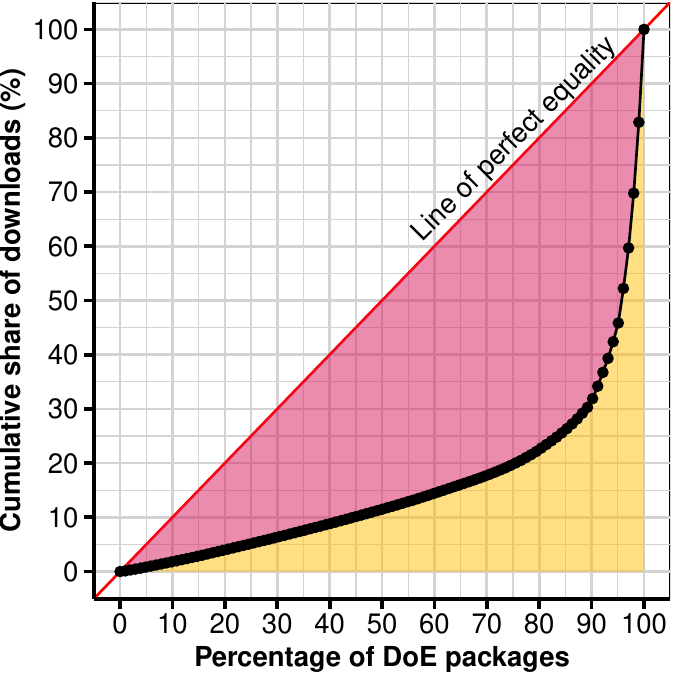
\includegraphics{figures/plot-lorenz-1} 

}

\caption{Lorenz curve of the total download count for DoE packages in 2021. The red line corresponds to the line of perfect equality. The yellow region shows the area under the Lorenz curve and the red region shows the area of the gap in equality.}\label{fig:plot-lorenz}
\end{figure}

If we consider package downloads as a measure of ``wealth'', then we can consider using the Gini index (Gini 1921) as a measure of download inequality across packages. The ratio of the red region to the total colored regions in Figure \ref{fig:plot-lorenz} corresponds to the Gini index for 2021. A Gini index of 0\% indicates equality in downloads across packages, whereas a value of 100\% indicates maximal inequality (all downloads are due to one package). In Figure \ref{fig:download-share}, we see that the distributions of the package downloads each year have a heavy right tail, with the Gini index ranging from 32.7\% to 69.1\% across the years 2013 to 2021, indicating that there is a high level of inequality in package downloads, particularly with more pronounced inequality in the last six years.

\begin{figure}[htbp]

{\centering 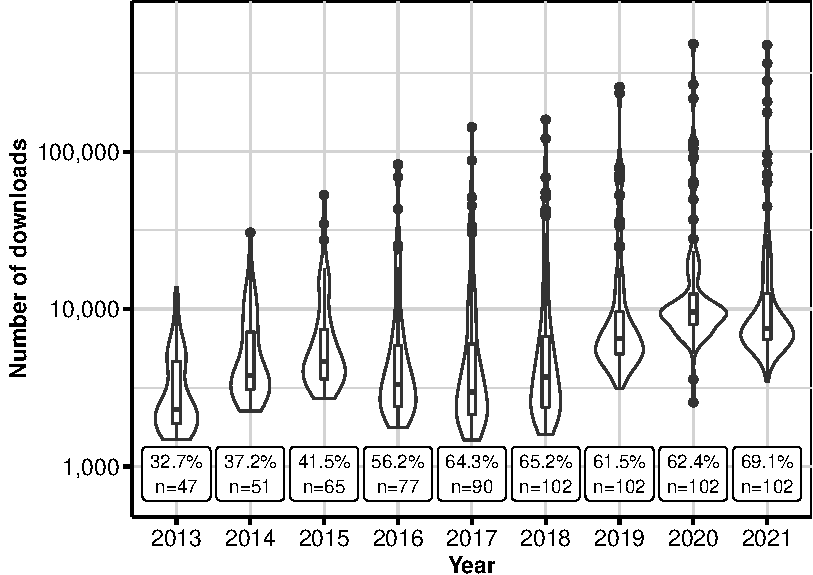
\includegraphics{figures/download-share-1} 

}

\caption{Distribution of number of downloads for DoE packages by year. Packages were removed in any year if they were released in that year or later so that each download count was for the full year. The label at the bottom of the plot shows the Gini index for downloads and the number of packages with a full download count in the corresponding year. In the last six years, the Gini index has consistently exceeded 60\%, indicating that most downloads are due to a relatively small number of packages. }\label{fig:download-share}
\end{figure}

An increase in the number of packages that are not highly downloaded may mean that \textbf{\emph{there are more packages to construct niche experimental designs}}. Some examples of these packages include \CRANpkg{qtlDesign}, \CRANpkg{PwrGSD} and \CRANpkg{Crossover} made for QTL experiments, group sequential designs and crossover trials, respectively. These packages would naturally have fewer potential users. Counterfactual to this, the increase could be due to other external factors, such as an increase in the number of skilled developers (and thus more package contributions), a change in CRAN policy or management to add packages (either to CRAN and/or task view), and/or the fact that new packages are still yet to amass users. While there is an argument that low download counts are due to the low utility and/or quality of packages, packages in CRAN task views are selected by expert maintainers. We can reasonably assume that any package listed in the CRAN task view has an acceptable utility and quality.

If the downloads are reflective of the experimental designs used in practice, \textbf{\emph{a small set of packages appears to be sufficient for most users to construct the full set of designs of experiments they need in practice}}. Packages of course evolve, and the top downloaded packages have had regular updates that may have broadened their scope from their previous releases.

While in absolute terms the Gini index is high for the \ctv{ExperimentalDesign} task view (32.7\% to 69.1\%), the inequality is not as severe as in other CRAN task views, as shown in Figure \ref{fig:fig-gini-all-ctvs}. We can see in Figure \ref{fig:fig-gini-all-ctvs} that the Gini index generally increases over time for DoE packages (as is generally the case for other CRAN task views, as shown in Figure S1 in the Supplementary Materials), but most other CRAN task views have a Gini index of over 75\%. This suggests that other CRAN task views may have dominant standards, and in comparison to other topics, there are more \textbf{\emph{diverse approaches to designing experiments}}, and thus, no single DoE package is dominant. However, this observation does not consider other approaches to generate experimental designs, such as the proprietary software CycDesignN (Whittaker, Williams, and John 2022), which may be widely used.

\begin{figure}[htbp]

{\centering 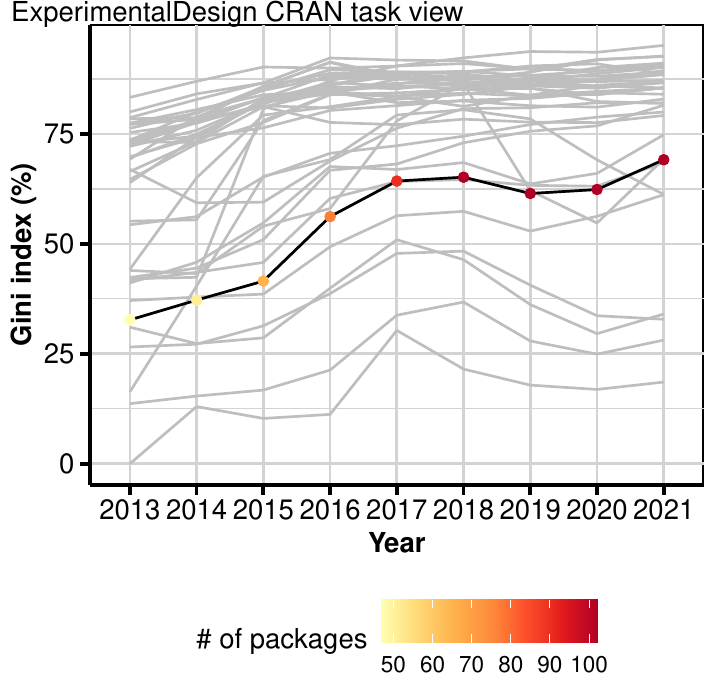
\includegraphics{figures/fig-gini-all-ctvs-1} 

}

\caption{The points show the Gini index of the download counts by year for the ExperimentalDesign task view with the color showing the number of packages. The gray lines show the line plots of the Gini index across years for all other CRAN task views. See Figure S1 in the Supplementary Material for the line graph of the Gini index across years for each CRAN task view.}\label{fig:fig-gini-all-ctvs}
\end{figure}

\hypertarget{the-field-of-experimental-design-is-slow-changing}{%
\subsection{The field of experimental design is slow-changing}\label{the-field-of-experimental-design-is-slow-changing}}

We can see in Figure \ref{fig:rank-over-time} that most of the top 10 ranking packages have been in the top 10 for the last nine years, with \CRANpkg{lhs} steadily climbing up the ranks in the last few years. It should be noted that the download of one package can prompt the download of another package; the most notable package connection is \CRANpkg{AlgDesign} and \CRANpkg{agricolae}, where the former is an import for the latter. The full network of package connections within the DoE packages is shown in Figure \ref{fig:plot-doe-network}.

\begin{figure}[htbp]

{\centering 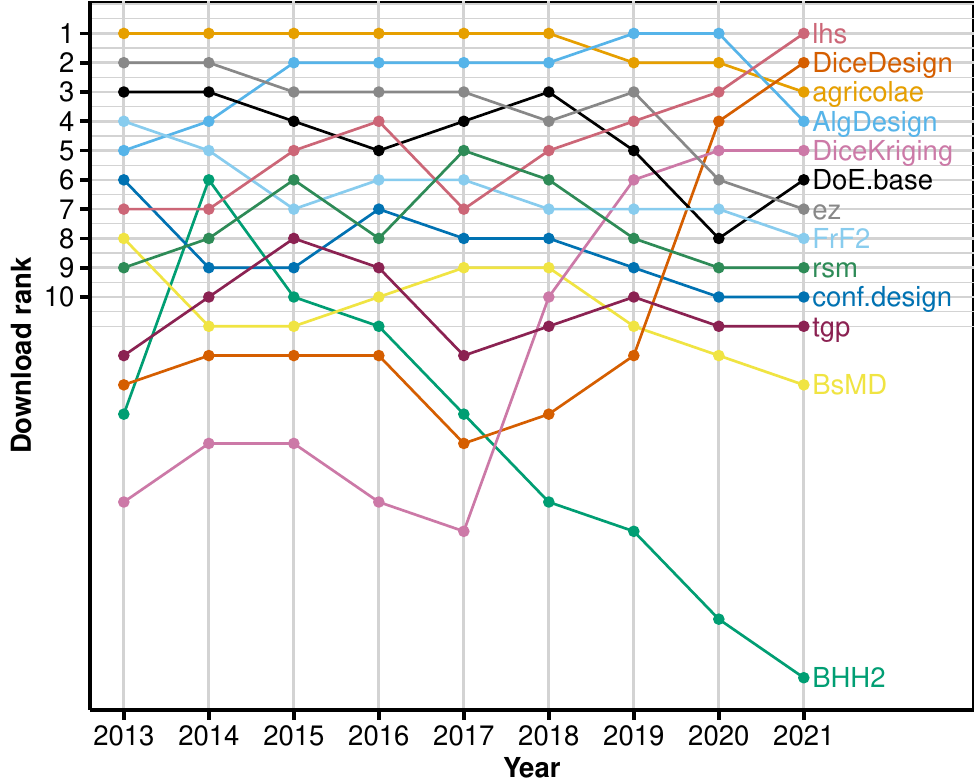
\includegraphics{figures/rank-over-time-1} 

}

\caption{The plot shows the rank of the top 10 packages downloaded by year. Packages that did not appear in the top 10 for at least two periods were omitted from the plot. Most packages are consistently in the top 10 for the period shown.}\label{fig:rank-over-time}
\end{figure}

Figure \ref{fig:release-date-vs-download} shows a moderate negative correlation between the first release date and the (log of) total download counts of DoE packages for any given year from 2013 to 2021. This suggests that packages released earlier are more likely to be used today (possibly for legacy reasons or the general inertia to adopt new packages). We can also see in Figure \ref{fig:release-date-vs-download} that most downloaded packages were released from 2004 to 2010.

\begin{figure}[htbp]

{\centering 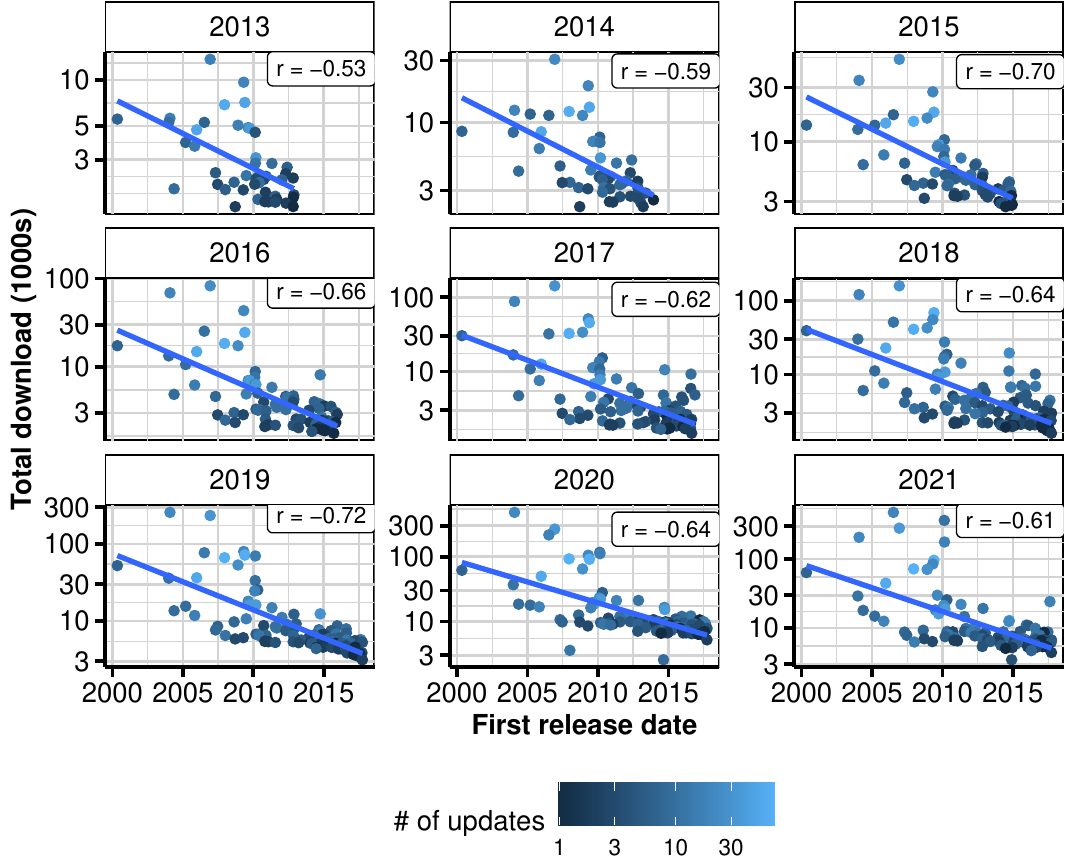
\includegraphics{figures/release-date-vs-download-1} 

}

\caption{The above figure shows the total download (in log scale) of a package in the corresponding year against the first release date of the package. The blue line corresponds to the least-squares fit of the simple linear regression model. The label in the upper right-hand corner shows the sample correlation coefficient between the first release date and log (with base 10) of the total download count. The high leverage point on the far left belongs to `conf.design`, authored by one of the earlier contributors to R.}\label{fig:release-date-vs-download}
\end{figure}

The consistency in the top 10 ranking packages (Figure \ref{fig:rank-over-time}) and the fact that most downloaded DoE packages were first released more than 10 years ago (Figure \ref{fig:release-date-vs-download}) indicate that either the existing packages fulfilled the needs of the masses in practice or no new packages were compelling for many to switch their practice. However, we also see that the top downloaded packages generally have more updates (see Figure \ref{fig:release-date-vs-download}); therefore, it is possible that the packages have improved or broadened the scope of their usage.

\hypertarget{optimal-designs-are-of-interest}{%
\subsection{Optimal designs are of interest}\label{optimal-designs-are-of-interest}}

Figure \ref{fig:wordcloud-over-time} shows some of the common purposes of DoE packages, based on bigrams in the package title and description. We only show the bigrams as unigrams were not insightful, and there were not many trigrams common across packages. To count the bigrams, we processed the text data as follows:

\begin{enumerate}
\def\labelenumi{\arabic{enumi}.}
\tightlist
\item
  We standardized the words to lower case and removed pluralization.
\item
  Multiple mentions of the same bigram within a package were counted as one (for example, \CRANpkg{AlgDesign} mentions ``experimental design'' four times in the title and the description, but this is counted as one).
\item
  Bigrams consisting of stop words were removed. The stop words are sourced from the lexicons in \texttt{tidytext::stop\_words} in addition to other words we deemed irrelevant, e.g., ``provide'', ``e.g.'', ``calculate'' and so on -- the full list is shown in the code provided in the link under \hyperref[pkgs]{Acknowledgment}.
\end{enumerate}

Unsurprisingly, the bigram ``experimental design'' was the most common. More interestingly, ``optimal design'' and ``sequential design'' appeared across different packages (indicated by the size of the word in Figure \ref{fig:wordcloud-over-time}), and the bigrams ``latin hypercube'' and ``computer experiment'' are used across a few packages that are downloaded frequently (indicated by the color of the word in Figure \ref{fig:wordcloud-over-time}). Sequential design, Latin hypercube sampling, and computer experiments (which generally include space-filling designs such as Latin hypercube sampling) generally operate by optimizing a user-selected criterion and can be classified as optimal designs.

\begin{figure}[htbp]

{\centering 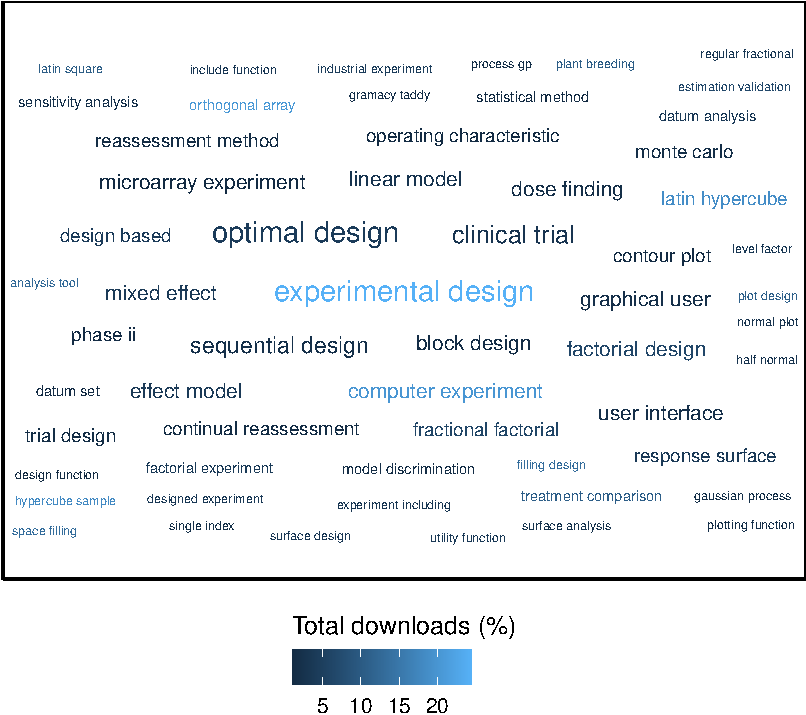
\includegraphics{figures/wordcloud-over-time-1} 

}

\caption{The above figure shows the word cloud of bigrams from the title and descriptions of the DoE packages. The size shows how often the bigram appears across the DoE packages and the color is relative to the total download count in 2021 for the packages that contain the bigram.}\label{fig:wordcloud-over-time}
\end{figure}

Although there exists a separate \ctv{ClinicalTrials} task view, the DoE packages clearly include some packages that are of interest to clinical trials, as shown by the size of the bigram ``clinical trial'' (and related bigrams like ``dose finding'' and ``phase ii'') in Figure \ref{fig:wordcloud-over-time}.

\hypertarget{development-of-experimental-designs-occur-in-silos}{%
\subsection{Development of experimental designs occurs in silos}\label{development-of-experimental-designs-occur-in-silos}}

Figure \ref{fig:ctv-summ-plot} shows that the \ctv{ExperimentalDesign} task view has the lowest average number of contributors among all the 39 CRAN task views. In addition, we can also see in Figure \ref{fig:ctv-summ-plot} that the \ctv{ExperimentalDesign} task view has one of the least intra-connectivity (the percentage of packages that make use of other packages within the same task view). The full connection between DoE packages is shown in Figure \ref{fig:plot-doe-network}. These observations suggest that \textbf{\emph{experimental design is one of the least collaborative fields}} and package development generally occurs in silos.

\begin{figure}[htbp]

{\centering 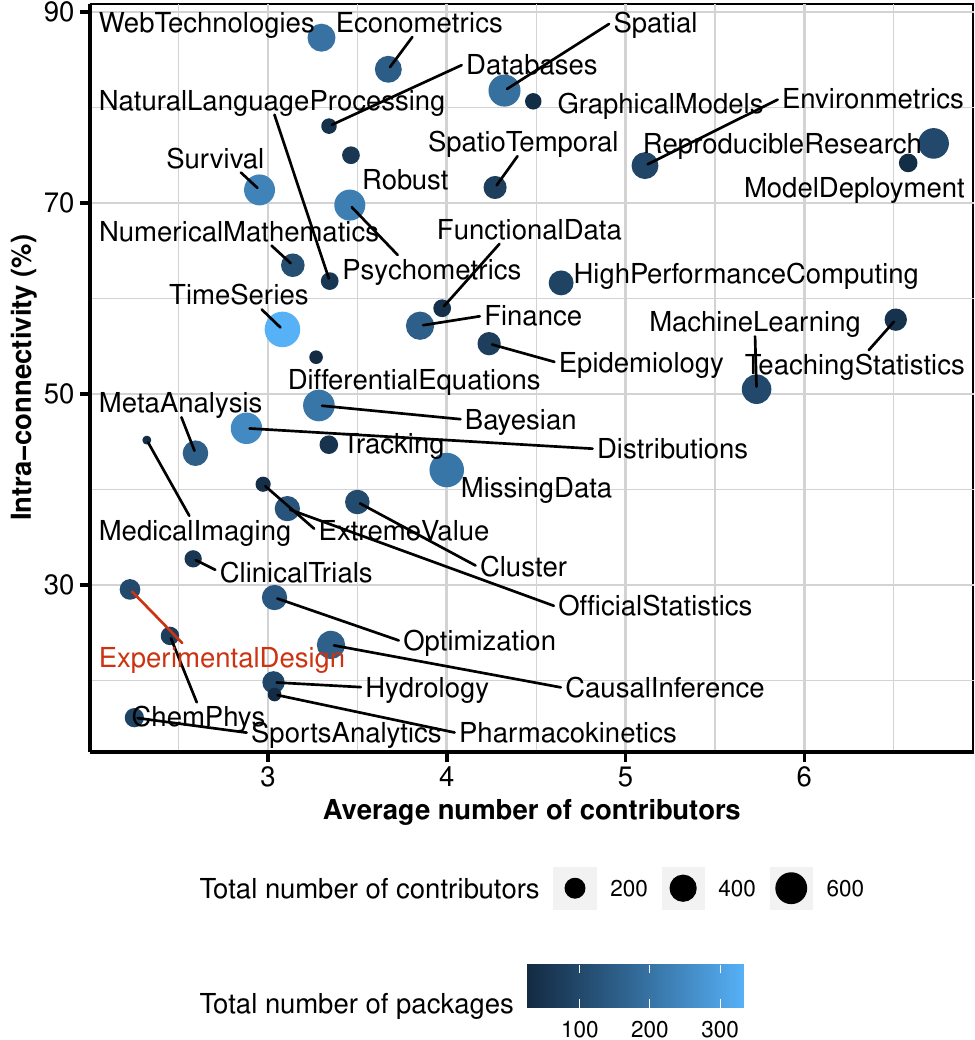
\includegraphics{figures/ctv-summ-plot-1} 

}

\caption{The above figure is a scatterplot of intra-connectivity (the percentage of packages that depend, suggest, or import at least one other package within the same task view) and the average number of contributors for each CRAN task view. Low intra-connectivity suggests that development within the topic mostly occurs in silos, while high intra-connectivity suggests that there are more interactions within the topic. The color shows the number of packages, the size of the point corresponds to the total number of contributors, and the text labels show the CRAN task view names.  The label of the ExperimentalDesign task view is colored in red. The task views in the bottom-left corner are topics that are more indicative of contributors working in silos. The actual numerical values are listed in Table S1 in the Supplementary Material.}\label{fig:ctv-summ-plot}
\end{figure}

\begin{figure}[htbp]

{\centering 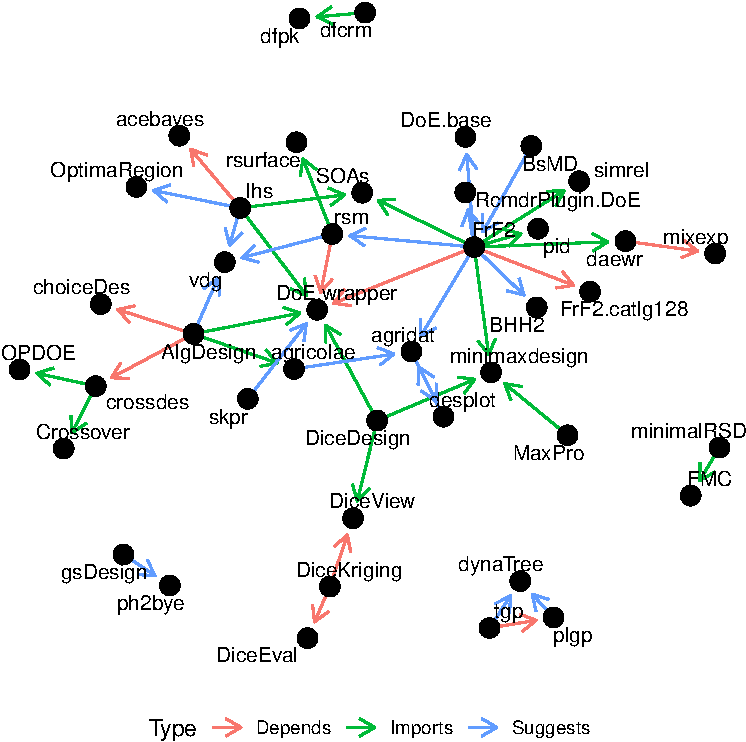
\includegraphics{figures/plot-doe-network-1} 

}

\caption{Package connections (depends, suggests, and imports) within DoE packages. The direction of the arrow shows the connection of packages, where the package on the tail of the arrow is a dependency, suggestion, or import for the package on the head of the arrow.  DoE packages that do not depend, suggest, or import another DoE package are not shown.}\label{fig:plot-doe-network}
\end{figure}

\hypertarget{design}{%
\section{Interface design}\label{design}}

In software design, there are two interface designs to consider: user interface (UI) and application programming interface (API). The UI is concerned with the interaction of the software by the user, while the API is concerned with how different programs interact and is predominantly of interest to the developer. The UI design is an abstraction that specifies the desired experimental design, and its choices enable how a user expresses the specification of an experimental design. The API design aids other developers in leveraging existing systems.

In this section, we discuss the interface designs of functions that output an experimental design based on three broad areas: factorial, recipe, and augmenting designs. The discussion is exclusive to the top downloaded packages (shown in Figure \ref{fig:rank-over-time}), with the exception of \CRANpkg{ez} and \CRANpkg{DiceKriging}, as the former is predominantly visualization of experimental data and the latter is about the analysis of computer experiments in addition to belonging to the same suite of packages as \CRANpkg{DiceDesign} (Dupuy, Helbert, and Franco 2015).

\hypertarget{the-case-of-factorial-designs}{%
\subsection{The case of factorial designs}\label{the-case-of-factorial-designs}}

Factorial experiments offer a challenge in allocating the treatment factors to experimental units, where the full set of factorial treatments cannot be administered (and replicated), and/or the experimental units have a grouping structure. The effort to address this challenge is reflected in the number of packages that focus on the construction of factorial designs, as described next.

The \CRANpkg{DoE.base} package (Grömping 2018) can construct full factorial and (regular and irregular) orthogonal array designs via \texttt{fac.design()} and \texttt{oa.design()}, respectively. The \CRANpkg{FrF2} package (Grömping 2014) constructs regular fractional 2-level factorial designs using \texttt{FrF2()} and \texttt{FrF2Large()}, with the latter for large designs. The \CRANpkg{conf.design} package (Venables 2013) constructs symmetric confounded factorial designs via \texttt{conf.design()} and the \CRANpkg{BHH2} package (Barrios 2016) generates a full or fractional 2-level factorial design matrix via \texttt{ffDesMatrix()}.

While the argument names and underlying algorithms of these functions to generate factorial designs differ, it generally requires the users to input the number of:

\begin{itemize}
\tightlist
\item
  treatment factors,
\item
  experimental runs (or replications), and
\item
  levels for each factor if the design was allowed to vary in the number of levels.
\end{itemize}

The output of the design is either a special class of list (e.g., the \texttt{design} class for \CRANpkg{DoE.base} and \CRANpkg{FrF2}) or a \texttt{data.frame} for \CRANpkg{conf.design} or a matrix for \texttt{BHH2}, such that an element or column corresponds to a treatment factor with each value corresponding to one experimental run. The treatment factors are generally assigned pseudo names (e.g., letters of the alphabet) or an argument exists for users to input treatment names as a character vector.

Some forms of factorial design are known by other names. For example, \emph{response surface designs} are factorial designs where the treatment factors are discrete levels of continuous variables. Two types of response surface designs can be constructed using the \CRANpkg{rsm} package (Lenth 2009): Box-Behnken design (Box and Behnken 1960) and central-composite designs (Box and Wilson 1951) via functions \texttt{bbd()} and \texttt{ccd()}, respectively, where the minimum required input is the number of factors. Another form of factorial design is the \emph{saturated designs}, where higher-order interaction effects of treatment factors are typically confounded with the main effects. Plackett-Burman designs (Plackett and Burman 1946) are a type of saturated design that can be generated by the function \texttt{pb()} in the \CRANpkg{FrF2} package, where the user provides the number of experimental runs and the number of treatment factors.

\hypertarget{the-case-of-recipe-designs}{%
\subsection{The case of recipe designs}\label{the-case-of-recipe-designs}}

The \CRANpkg{agricolae} package (de Mendiburu 2021) is the prime example of constructing designs based on a set of so-called ``recipe functions'', where each function corresponds to a single class of experimental design. For example, \texttt{design.crd()}, \texttt{design.rcbd()}, and \texttt{design.split()} construct completely randomized, randomized complete block, and split-plot designs, respectively. Users typically supply treatment labels (or the number of treatments in the case of \texttt{design.split()}) and the number of replications as arguments for these functions. The output is a list with one element corresponding to a \texttt{data.frame} that contains the design in a table such that the row corresponds to the experimental run and the columns correspond to the experimental variables (we refer to this format simply as ``table format'' henceforth).

The use of recipe functions is not limited to classical experimental designs; the \CRANpkg{AlgDesign} (Wheeler 2022) package offers three primary functions for generating optimal designs: \texttt{optBlock()}, \texttt{optFederov()}, and \texttt{optMonteCarlo()}. In general, these functions require data and formulas in terms of the supplied data variables, along with the choice of the criterion (e.g., the D-criterion), with the output as a list with one element corresponding to the design in a table format. The difference between these functions lies in the underlying search strategy for optimal designs, and the name of the function is a surrogate for the search algorithm.

Computer experiments, which generally involve space-filling designs, are implemented in packages such as \CRANpkg{lhs} (Carnell 2022) and \CRANpkg{DiceDesign} (Dupuy, Helbert, and Franco 2015). For the \CRANpkg{lhs} package, functions such as \texttt{randomLHS()}, \texttt{optimumLHS()}, and \texttt{maximinLHS()} require users to specify the sample size (\(n\)) and the number of variables (\(p\)). It generates a Latin hypercube sample (McKay, Beckman, and Conover 1979) based on different optimization schemes (in this case, random, S-optimal, and maxmin criteria, respectively; see package documentation for more details). Similarly, for \CRANpkg{DiceDesign}, there is a comprehensive list of space-filling designs such as \texttt{dmaxDesign()}, \texttt{lhsDesign()}, and \texttt{wspDesign()} with input of \(n\) and \(p\) as before (among additional parameters for some) that implement algorithms that either maximize the entropy (Shewry and Wynn 1987), produce a random Latin hypercube sample, or use the WSP algorithm (Santiago, Claeys-Bruno, and Sergent 2012), respectively. These designs output an \(n \times p\) matrix with values between 0 and 1. Again, these functions employ a recipe style, in which each function has a name that corresponds to a certain search strategy to generate the experimental design.

\hypertarget{the-case-of-augmenting-designs}{%
\subsection{The case of augmenting designs}\label{the-case-of-augmenting-designs}}

Some functions in the DoE packages require the input of existing experimental designs to produce new designs. For example, the \CRANpkg{DoE.base} package contains some experimental functions, \texttt{cross.design()} and \texttt{param.design()}, to combine designs, with the former taking a Cartesian product of the input designs, while the latter uses a Taguchi style (Taguchi 1986) to aggregate the designs with the inner and outer arrays. The \CRANpkg{lhs} package contains a function, \texttt{augmentLHS()}, to add additional samples to the existing Latin hypercube sample.

Another class of augmenting design is \emph{sequential design} (also called \emph{adaptive sampling}), which is best represented by \CRANpkg{tgp} (Gramacy and Taddy 2010). This requires prior information that is used to inform the next experimental design using \texttt{tgp.design()} and \texttt{dopt.gp()}. The user is required to supply candidate samples to subsample from and a model or a prior experimental design. Follow-up experiments, which can also be classified as sequential designs, are implemented by \CRANpkg{BsMD} (Barrios 2020) using a model-discriminant approach with \texttt{MD()}.

\hypertarget{discussion}{%
\section{Discussion}\label{discussion}}

Through the exploratory data analysis of the three data sources (package download logs, package metadata, and CRAN task views) outlined in \hyperref[data]{Data}, we observed in \hyperref[eda]{Exploratory data analysis} that the total download of DoE packages is concentrated only on a handful of R-packages, although these represent a diverse set in comparison with other CRAN task views. Furthermore, the data suggest that experimental design is the least collaborative field.

There are a number of limitations and shortcomings to our exploratory data analysis. First, CRAN task views are volunteer maintained, so some experimental design packages may not be included in the DoE packages. Second, we used only the RStudio CRAN mirror download, which may have biased our observations. Third, our analysis was limited to R-packages alone, and many practitioners may use other methods to construct experimental designs. Finally, all our statements should be treated as speculative rather than conclusive; the data are all observational, so no conclusive, generalizable statement is possible. Regardless, the data-driven nature of our analysis provides objective insight into the field of experimental design.

The interface design (discussed in \hyperref[design]{Interface design}) reveals that the most widely used DoE packages generally have functions that 1) focus on certain aspects of experimental design (e.g., factorial structure or augmenting design), 2) are in a recipe format (i.e., the name of the function is a surrogate for a single class of the design or optimal search algorithm), and 3) context is often a second thought -- many inputs are a single integer corresponding to the number of factors, levels, or experimental runs (or sample size). The function will often assign pseudo-factor names, or there is an optional argument to input a character vector that corresponds to the factor names. These interface designs require users to have processed the experiment in statistical terms (often stripping the experimental context away) and simultaneously, users must choose the generation mechanism by selecting an appropriate function. Arguably, the current dominant interface designs are not aligned with the way practitioners cognitively design their experiments. Often, the critical part of designing an experiment is to understand the experimental structure, and the experimental context can govern or guide the choice of algorithm to allocate treatments. In addition, the nature of recipe functions can obscure the understanding and relation of designs (e.g., how do you go from an unstructured factorial design to a split plot design?). Each new method for generating an experimental design appears to correspond to a completely new function, and intermediate results are often not easily accessible. These factors may contribute to why developers often work in silos in the field of experimental design.

A consistent cognitive interface design that leverages existing developments and can be easily extended to new methods will conceivably be of great help to practitioners. Some efforts to this end are seen in \CRANpkg{DoE.wrapper} (Grömping 2020), which contains wrapper recipe functions for other DoE packages such as \CRANpkg{lhs}, \CRANpkg{AlgDesign}, and \CRANpkg{FrF2} (see Figure \ref{fig:plot-doe-network}), and is also the subject of the developmental package \CRANpkg{edibble} (Tanaka 2021). Undoubtedly, no single developer or package can cater to all experimental designs; therefore, any unifying interface should consider how other developers can contribute or add their methods. Future research could benefit from further exploratory data analysis, expanding the study beyond R-packages, and discussing other aspects of interface designs.

\hypertarget{pkgs}{%
\section{Acknowledgment}\label{pkgs}}

This paper uses \CRANpkg{targets} (Landau 2021) and \CRANpkg{renv} (Ushey 2022) for reproducibility, \CRANpkg{knitr} (Xie 2015) and \CRANpkg{rmarkdown} (Xie, Allaire, and Grolemund 2018) for creating reproducible documents, \CRANpkg{ggplot2} (Wickham 2016), \CRANpkg{ggraph} (Pedersen 2021), \CRANpkg{ggwordcloud} (Le Pennec and Slowikowski 2019) and \texttt{colorspace} (Zeileis et al. 2020) for visualization, \CRANpkg{kableExtra} (Zhu 2021) for customizing the table in the Supplementary Material, and \CRANpkg{tidyverse} (Wickham et al. 2019), \CRANpkg{tidytext} (Silge and Robinson 2016), \CRANpkg{pluralize} (Rudis and Embrey 2020), and \CRANpkg{ineq} (Zeileis 2014) for data processing and manipulation, and \CRANpkg{cranlogs} (Csárdi 2019) and \CRANpkg{ctv} (Zeileis 2005) for extracting data. All codes used to reproduce this paper are found in \url{https://github.com/emitanaka/paper-DoE-review}.

\hypertarget{references}{%
\section*{References}\label{references}}
\addcontentsline{toc}{section}{References}

\hypertarget{refs}{}
\begin{CSLReferences}{1}{0}
\leavevmode\vadjust pre{\hypertarget{ref-BHH2}{}}%
Barrios, Ernesto. 2016. \emph{BHH2: Useful Functions for Box, Hunter and Hunter II}. \url{https://CRAN.R-project.org/package=BHH2}.

\leavevmode\vadjust pre{\hypertarget{ref-BsMD}{}}%
---------. 2020. \emph{BsMD: Bayes Screening and Model Discrimination}. \url{https://CRAN.R-project.org/package=BsMD}.

\leavevmode\vadjust pre{\hypertarget{ref-Box1960-wr}{}}%
Box, G E P, and D W Behnken. 1960. {``Some New Three Level Designs for the Study of Quantitative Variables.''} \emph{Technometrics: A Journal of Statistics for the Physical, Chemical, and Engineering Sciences} 2 (4): 455--75. \url{https://doi.org/10.2307/1266454}.

\leavevmode\vadjust pre{\hypertarget{ref-Box1951-ji}{}}%
Box, G E P, and K B Wilson. 1951. {``On the Experimental Attainment of Optimum Conditions.''} \emph{Journal of the Royal Statistical Society. Series B, Statistical Methodology} 13 (1): 1--45.

\leavevmode\vadjust pre{\hypertarget{ref-lhs}{}}%
Carnell, Rob. 2022. \emph{Lhs: Latin Hypercube Samples}. \url{https://CRAN.R-project.org/package=lhs}.

\leavevmode\vadjust pre{\hypertarget{ref-cranlogs}{}}%
Csárdi, Gábor. 2019. \emph{Cranlogs: Download Logs from the 'RStudio' 'CRAN' Mirror}. \url{https://CRAN.R-project.org/package=cranlogs}.

\leavevmode\vadjust pre{\hypertarget{ref-agricolae}{}}%
de Mendiburu, Felipe. 2021. \emph{Agricolae: Statistical Procedures for Agricultural Research}. \url{https://CRAN.R-project.org/package=agricolae}.

\leavevmode\vadjust pre{\hypertarget{ref-DiceDesign}{}}%
Dupuy, Delphine, Céline Helbert, and Jessica Franco. 2015. {``{DiceDesign} and {DiceEval}: Two {R} Packages for Design and Analysis of Computer Experiments.''} \emph{Journal of Statistical Software} 65 (11): 1--38. \url{https://www.jstatsoft.org/v65/i11/}.

\leavevmode\vadjust pre{\hypertarget{ref-Fisher1935-qc}{}}%
Fisher, Ronald. 1935. \emph{The Design of Experiments}. Oliver; Boyd.

\leavevmode\vadjust pre{\hypertarget{ref-Gini1921-mf}{}}%
Gini, Corrado. 1921. {``Measurement of Inequality of Incomes.''} \emph{The Economic Journal} 31 (121): 124--26. \url{https://doi.org/10.2307/2223319}.

\leavevmode\vadjust pre{\hypertarget{ref-tgp}{}}%
Gramacy, Robert B., and Matthew Taddy. 2010. {``Categorical Inputs, Sensitivity Analysis, Optimization and Importance Tempering with {tgp} Version 2, an {R} Package for Treed Gaussian Process Models.''} \emph{Journal of Statistical Software} 33 (6): 1--48. \url{https://doi.org/10.18637/jss.v033.i06}.

\leavevmode\vadjust pre{\hypertarget{ref-FrF2}{}}%
Grömping, Ulrike. 2014. {``{R} Package {FrF2} for Creating and Analyzing Fractional Factorial 2-Level Designs.''} \emph{Journal of Statistical Software} 56 (1): 1--56. \url{https://www.jstatsoft.org/v56/i01/}.

\leavevmode\vadjust pre{\hypertarget{ref-DoE.base}{}}%
---------. 2018. {``{R} Package {DoE.base} for Factorial Experiments.''} \emph{Journal of Statistical Software} 85 (5): 1--41. \url{https://doi.org/10.18637/jss.v085.i05}.

\leavevmode\vadjust pre{\hypertarget{ref-DoE.wrapper}{}}%
---------. 2020. \emph{DoE.wrapper: Wrapper Package for Design of Experiments Functionality}. \url{https://CRAN.R-project.org/package=DoE.wrapper}.

\leavevmode\vadjust pre{\hypertarget{ref-targets}{}}%
Landau, William Michael. 2021. {``The Targets r Package: A Dynamic Make-Like Function-Oriented Pipeline Toolkit for Reproducibility and High-Performance Computing.''} \emph{Journal of Open Source Software} 6 (57): 2959. \url{https://doi.org/10.21105/joss.02959}.

\leavevmode\vadjust pre{\hypertarget{ref-ggwordcloud}{}}%
Le Pennec, Erwan, and Kamil Slowikowski. 2019. \emph{Ggwordcloud: A Word Cloud Geom for 'Ggplot2'}. \url{https://CRAN.R-project.org/package=ggwordcloud}.

\leavevmode\vadjust pre{\hypertarget{ref-rsm}{}}%
Lenth, Russell V. 2009. {``Response-Surface Methods in {R}, Using {rsm}.''} \emph{Journal of Statistical Software} 32 (7): 1--17. \url{https://doi.org/10.18637/jss.v032.i07}.

\leavevmode\vadjust pre{\hypertarget{ref-Lorenz1905-tc}{}}%
Lorenz, M O. 1905. {``Methods of Measuring the Concentration of Wealth.''} \emph{Publications of the American Statistical Association} 9 (70): 209--19. \url{https://doi.org/10.2307/2276207}.

\leavevmode\vadjust pre{\hypertarget{ref-McKay1979-aw}{}}%
McKay, M D, R J Beckman, and W J Conover. 1979. {``Comparison of Three Methods for Selecting Values of Input Variables in the Analysis of Output from a Computer Code.''} \emph{Technometrics: A Journal of Statistics for the Physical, Chemical, and Engineering Sciences} 21 (2): 239--45. \url{https://doi.org/10.1080/00401706.1979.10489755}.

\leavevmode\vadjust pre{\hypertarget{ref-ggraph}{}}%
Pedersen, Thomas Lin. 2021. \emph{Ggraph: An Implementation of Grammar of Graphics for Graphs and Networks}. \url{https://CRAN.R-project.org/package=ggraph}.

\leavevmode\vadjust pre{\hypertarget{ref-Plackett1946-ly}{}}%
Plackett, R L, and J P Burman. 1946. {``The Design of Optimum Multifactorial Experiments.''} \emph{Biometrika} 33 (4): 302--25.

\leavevmode\vadjust pre{\hypertarget{ref-Pukelsheim2006-sv}{}}%
Pukelsheim, Friedrich. 2006. \emph{Optimal Design of Experiments}.

\leavevmode\vadjust pre{\hypertarget{ref-R}{}}%
R Core Team. 2021. \emph{R: A Language and Environment for Statistical Computing}. Vienna, Austria: R Foundation for Statistical Computing. \url{https://www.R-project.org/}.

\leavevmode\vadjust pre{\hypertarget{ref-python}{}}%
Rossum, G. van. 1995. {``Python Tutorial.''} CS-R9526. Amsterdam: Centrum voor Wiskunde en Informatica (CWI).

\leavevmode\vadjust pre{\hypertarget{ref-pluralize}{}}%
Rudis, Bob, and Blake Embrey. 2020. \emph{Pluralize: Pluralize and 'Singularize' Any (English) Word}. \url{https://CRAN.R-project.org/package=pluralize}.

\leavevmode\vadjust pre{\hypertarget{ref-Santiago2012-ui}{}}%
Santiago, J, M Claeys-Bruno, and M Sergent. 2012. {``Construction of Space-Filling Designs Using {WSP} Algorithm for High Dimensional Spaces.''} \emph{Chemometrics and Intelligent Laboratory Systems} 113 (April): 26--31. \url{https://doi.org/10.1016/j.chemolab.2011.06.003}.

\leavevmode\vadjust pre{\hypertarget{ref-sas1985sas}{}}%
SAS Institute. 1985. \emph{SAS User's Guide: Statistics}. Vol. 2. Sas Inst.

\leavevmode\vadjust pre{\hypertarget{ref-Shewry1987-jn}{}}%
Shewry, M C, and H P Wynn. 1987. {``Maximum Entropy Sampling.''} \emph{Journal of Applied Statistics} 14 (2): 165--70. \url{https://doi.org/10.1080/02664768700000020}.

\leavevmode\vadjust pre{\hypertarget{ref-tidytext}{}}%
Silge, Julia, and David Robinson. 2016. {``Tidytext: Text Mining and Analysis Using Tidy Data Principles in r.''} \emph{JOSS} 1 (3). \url{https://doi.org/10.21105/joss.00037}.

\leavevmode\vadjust pre{\hypertarget{ref-Taguchi1986-ut}{}}%
Taguchi, Genichi. 1986. \emph{Introduction to Quality Engineering: Designing Quality into Products and Processes}. Quality Resources.

\leavevmode\vadjust pre{\hypertarget{ref-edibble}{}}%
Tanaka, Emi. 2021. {``{edibble R-package}.''} \emph{GitHub Repository}. \url{https://github.com/emitanaka/edibble}; GitHub.

\leavevmode\vadjust pre{\hypertarget{ref-renv}{}}%
Ushey, Kevin. 2022. \emph{Renv: Project Environments}. \url{https://CRAN.R-project.org/package=renv}.

\leavevmode\vadjust pre{\hypertarget{ref-conf.design}{}}%
Venables, Bill. 2013. \emph{Conf.design: Construction of Factorial Designs}. \url{https://CRAN.R-project.org/package=conf.design}.

\leavevmode\vadjust pre{\hypertarget{ref-Wasserman1975-xr}{}}%
Wasserman, Anthony I. 1975. {``Issues in Programming Language Design - an Overview.''} In.

\leavevmode\vadjust pre{\hypertarget{ref-AlgDesign}{}}%
Wheeler, Bob. 2022. \emph{AlgDesign: Algorithmic Experimental Design}. \url{https://CRAN.R-project.org/package=AlgDesign}.

\leavevmode\vadjust pre{\hypertarget{ref-cycdesignn}{}}%
Whittaker, D., E. R. Williams, and J. A John. 2022. \emph{CycDesign: A Package for the Computer Generation of Experimental Designs,} (version 7.0). \url{https://vsni.co.uk/software/cycdesign}.

\leavevmode\vadjust pre{\hypertarget{ref-ggplot2}{}}%
Wickham, Hadley. 2016. \emph{Ggplot2: Elegant Graphics for Data Analysis}. Springer-Verlag New York. \url{https://ggplot2.tidyverse.org}.

\leavevmode\vadjust pre{\hypertarget{ref-Wickham2019-mj}{}}%
Wickham, Hadley, Mara Averick, Jennifer Bryan, Winston Chang, Lucy D'agostino McGowan, Romain Francois, Garrett Grolemund, et al. 2019. {``Welcome to the Tidyverse.''} \emph{Journal of Open Source Software} 4 (43): 1686.

\leavevmode\vadjust pre{\hypertarget{ref-knitr}{}}%
Xie, Yihui. 2015. \emph{Dynamic Documents with {R} and Knitr}. 2nd ed. Boca Raton, Florida: Chapman; Hall/CRC. \url{https://yihui.org/knitr/}.

\leavevmode\vadjust pre{\hypertarget{ref-rmarkdown}{}}%
Xie, Yihui, J. J. Allaire, and Garrett Grolemund. 2018. \emph{R Markdown: The Definitive Guide}. Boca Raton, Florida: Chapman; Hall/CRC. \url{https://bookdown.org/yihui/rmarkdown}.

\leavevmode\vadjust pre{\hypertarget{ref-ctv}{}}%
Zeileis, Achim. 2005. {``{CRAN} Task Views.''} \emph{R News} 5 (1): 39--40. \url{https://CRAN.R-project.org/doc/Rnews/}.

\leavevmode\vadjust pre{\hypertarget{ref-ineq}{}}%
---------. 2014. \emph{Ineq: Measuring Inequality, Concentration, and Poverty}. \url{https://CRAN.R-project.org/package=ineq}.

\leavevmode\vadjust pre{\hypertarget{ref-colorspace}{}}%
Zeileis, Achim, Jason C. Fisher, Kurt Hornik, Ross Ihaka, Claire D. McWhite, Paul Murrell, Reto Stauffer, and Claus O. Wilke. 2020. {``{colorspace}: A Toolbox for Manipulating and Assessing Colors and Palettes.''} \emph{Journal of Statistical Software} 96 (1): 1--49. \url{https://doi.org/10.18637/jss.v096.i01}.

\leavevmode\vadjust pre{\hypertarget{ref-kableExtra}{}}%
Zhu, Hao. 2021. \emph{kableExtra: Construct Complex Table with 'Kable' and Pipe Syntax}. \url{https://CRAN.R-project.org/package=kableExtra}.

\end{CSLReferences}

\bibliography{paper.bib}

\address{%
Emi Tanaka\\
Monash University\\%
Department of Econometrics and Business Statistics\\ Monash University, Clayton, VIC 3800\\
%
\url{https://emitanaka.org/}\\%
\textit{ORCiD: \href{https://orcid.org/0000-0002-1455-259X}{0000-0002-1455-259X}}\\%
\href{mailto:emi.tanaka@monash.edu}{\nolinkurl{emi.tanaka@monash.edu}}%
}

\address{%
Dewi Amaliah\\
Monash University\\%
Department of Econometrics and Business Statistics\\ Monash University, Clayton, VIC 3800\\
%
%
%
%
}

\end{article}


\end{document}
